\section*{Appendix A: Analytical Results}
\label{sec:appendixA}

\subsection*{Example 1}
\label{sec:example1Anal}

For the system described in Section~\ref{sec:example1} we have the following

\begin{align} 
  R_0   &= p_A + p_B p_C - p_A p_B p_C = 0.01495   \\
  R_A^- &= p_B p_C = 0.005  \\
  R_A^+ &= 1.0  \\
  R_B^- &= p_A = 0.01  \\
  R_B^+ &= p_A + p_C - p_A p_C = 0.109  \\
  R_C^- &= p_A = 0.01 \\
  R_C^+ &= p_A + p_B - p_A p_B = 0.0595  
\end{align}

Thus:
\begin{align} 
  FV_A &= \frac{R_0-R_A^-}{R_0} = 0.665552 \\
  FV_B &= \frac{R_0-R_B^-}{R_0} = 0.331104 \\
  FV_C &= \frac{R_0-R_C^-}{R_0} = 0.331104    
\end{align}
and:
\begin{align} 
  RAW_A &= \frac{R_i^+}{R_0} = 66.88963 \\
  RAW_B &= \frac{R_i^+}{R_0} = 7.29097 \\
  RAW_C &= \frac{R_i^+}{R_0} = 3.97993    
\end{align}

\subsection*{Example 2}
\label{sec:example2Anal}

We can solve the system described in Section~\ref{sec:example2} using reliability
block diagrams (see Fig.~\ref{fig:example2RBB}).

\begin{figure}
    \centering
    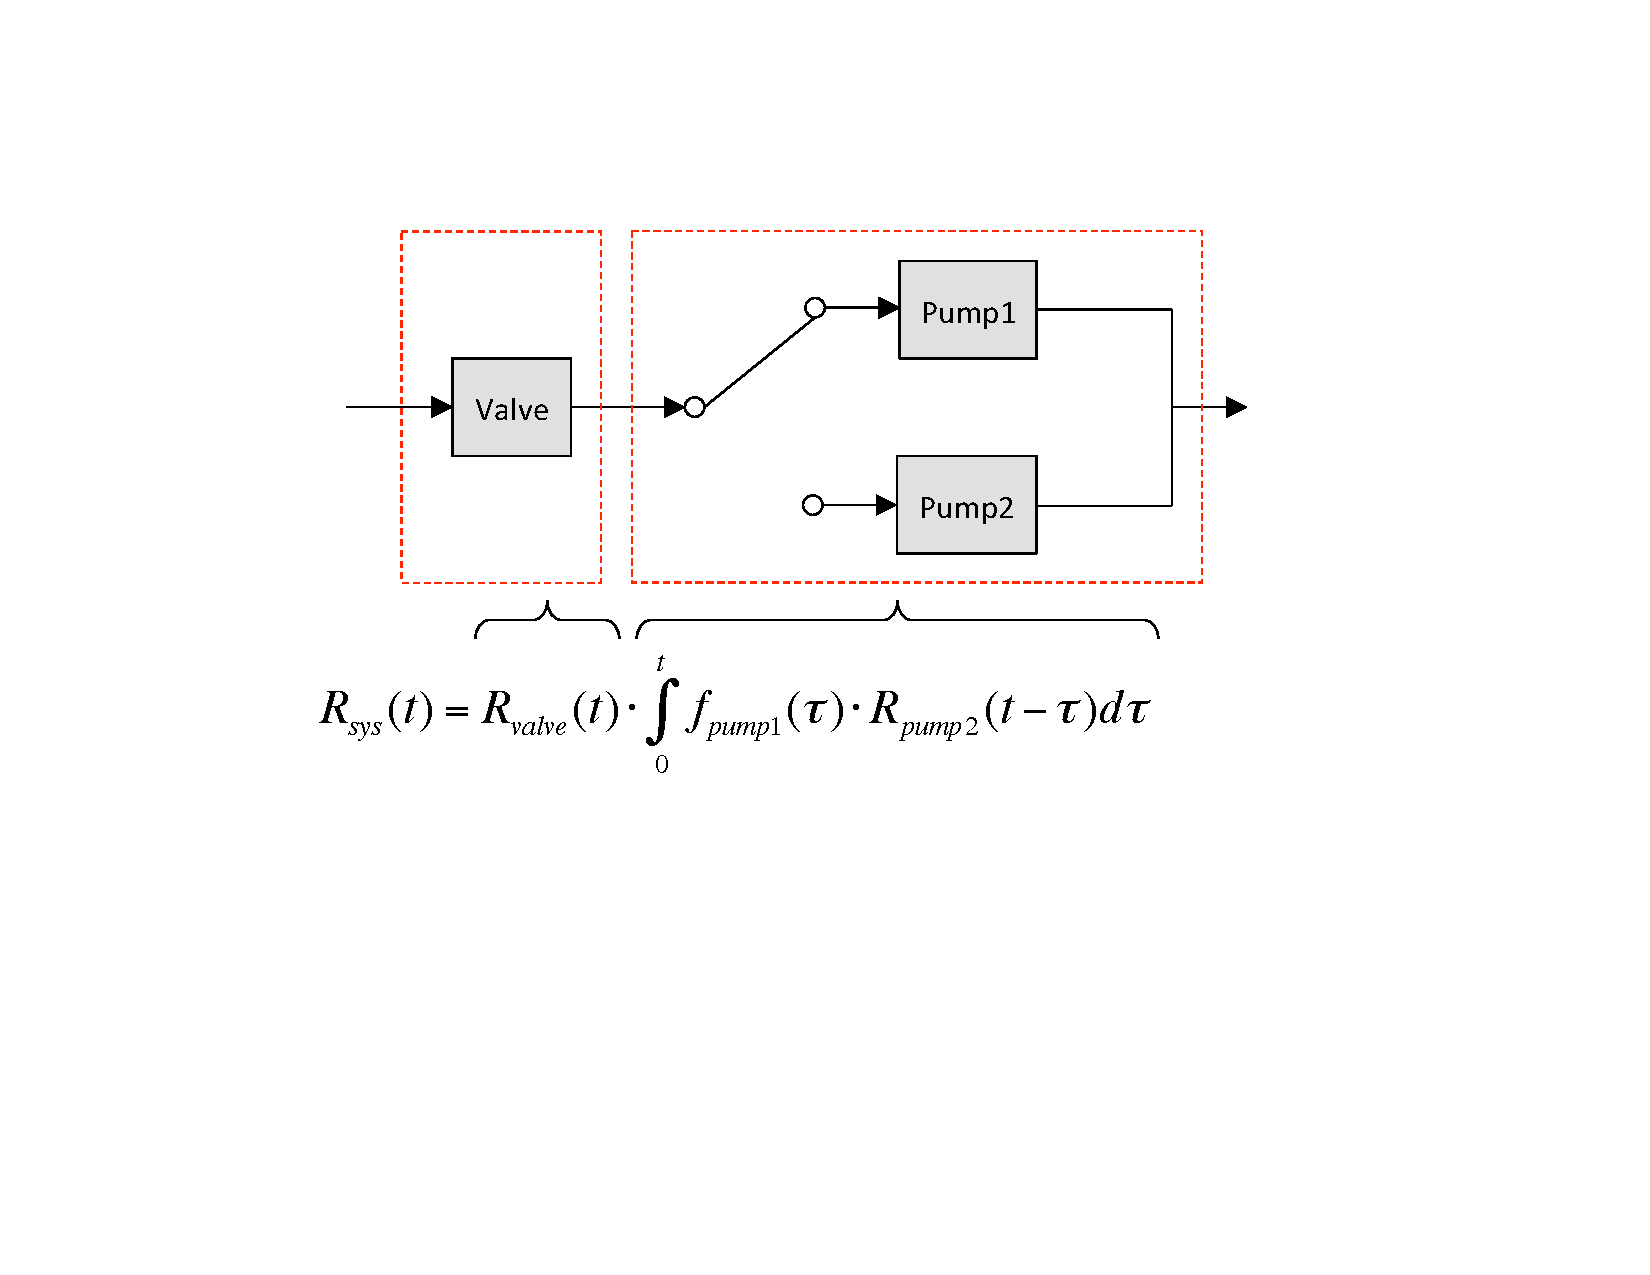
\includegraphics[scale=0.5]{blocks.pdf}
    \caption{Reliability block diagrams for Example 2 (see Section~\ref{sec:example2}).}
    \label{fig:example2RBB}
\end{figure}

Thus time dependent reliability of the system $R_sys(t)$ as function of time $t$:
\begin{equation}
  R_{sys}(t) = R_{valve}(t) \int_0^t f_{pump1}(\tau) R_{pump2}(t-\tau) d\tau
\end{equation}
where:
\begin{itemize}
  \item $R_{valve}(t) = e^{-\lambda_{valve} t}$
  \item $f_{pump1}(t) = \lambda_{pump1} e^{-\lambda_1 t}$
  \item $R_{pump2}(t) = e^{-\lambda_{pump2} t}$
\end{itemize}

It can be shown that if $\lambda_{pump1} = \lambda_{pump2} = \bar{\lambda}$:
\begin{equation}
  R_{sys}(t) = e^{-\lambda_{valve} t} [ e^{-\bar{\lambda}} (1+\bar{\lambda} t) ]
\end{equation}

For this system we have the following for a mission time $T=24$ hours:
\begin{align} 
  & R_0         = 1.0 - R_{sys}(T) = 0.85063876  \\
  & R_{valve}^- = 1.0 - [ e^{-\bar{\lambda} T} (1+\bar{\lambda} T) ] = 0.593994129 \\
  & R_{valve}^+ = 1.0  \\
  & R_{pump1}^- = 1.0 - R_{valve}(T) = 0.6321205  \\
  & R_{pump1}^+ = 1.0 - R_{valve}(T) R_{pump2}(T) = 0.95021292 \\
  & R_{pump2}^- = R_{pump1}^- = 0.6321205 \\
  & R_{pump2}^+ = R_{pump1}^+ = 0.95021292
\end{align}

\subsection*{Example 3}
\label{sec:example3Anal}

We can solve the system described in Section~\ref{sec:example2} using again reliability
block diagrams.
Thus time dependent reliability of the system $R_sys(t)$ as function of time $t$:
\begin{equation}
  R_{sys}(t) = R_{valve}(t) R_{2oo3}(t)
\end{equation}
where $R_{2oo3}(t)$ represents reliability of a set of three identical components 
in a 2 out of 3 (2oo3) configuration. 

It can be shown that if 
$\lambda_{pump1} = \lambda_{pump2} = \lambda_{pump3} = \bar{\lambda}$
(thus $R_{pump1}(t) = R_{pump2}(t) = R_{pump3}(t) = \bar{R}(t) = e^{- \bar{\lambda} t}$)
then $R_{2oo3}(t)$ can be written as
\begin{equation}
  R_{2oo3}(t) = \sum\limits_{n=2}^3 \binom{3}{n} \bar{R}(t)^n [1-\bar{R}(t)]^{3-n}
              = 3 e^{- 2 \bar{\lambda} t} (1 - e^{- \bar{\lambda} t}) + e^{- 3 \bar{\lambda} t}
\end{equation}

For this system we have the following for a mission time $T=24$ hours:
\begin{align} 
  & R_0         = 1.0 - R_{sys}(T) = 0.981609917 \\
  & R_{valve}^- = 1.0 - R_{2oo3}(T) = 0.95001058 \\
  & R_{valve}^+ = 1.0 \\
  & R_{pump1}^- = 1.0 - R_{1oo2}(T) R_{valve}(T) = 0.907163789\\
  & R_{pump1}^+ = 1.0 - R_{valve}(T) \bar{R}(t)^2 = 0.993262051\\
  & R_{pump2}^- = R_{pump1}^- \\
  & R_{pump2}^+ = R_{pump1}^+ \\
  & R_{pump3}^- = R_{pump1}^- \\
  & R_{pump3}^+ = R_{pump1}^+ 
\end{align}
where $R_{1oo2}(t)$ represents reliability of a set of two identical components 
in a 1 out of 2 (1oo2) configuration:

\begin{equation}
  R_{1oo2}(t) = \sum\limits_{n=1}^2 \binom{2}{n} \bar{R}(t)^n [1-\bar{R}(t)]^{2-n}
              = 2 e^{- \bar{\lambda} t} (1 - e^{- \bar{\lambda} t}) + e^{- 2 \bar{\lambda} t}
\end{equation}
